\section{课题来源及研究的目的和意义}

载脂蛋白A1 (ApoA1) 为附着于高密度脂蛋白(HDL)及乳靡小球上的载脂蛋白。
是构成血浆中高密度脂蛋白(HDL)蛋白质部分的主要成分。
ApoA1 在体内脂质代谢的角色相当重要,因此常被视为预测个体冠心病风险的生物标记。
ApoA1 还被用于癌症诊断\cite{limwjxtd}、预后预测\cite{apoayuhz}等方面有重要作用。
因此,利用分子动力学方法,模拟 ApoA1 的构象变化、折叠过程,对于生物医学、化学等研究有重要意义。


\begin{figure}[h]
    \centering
    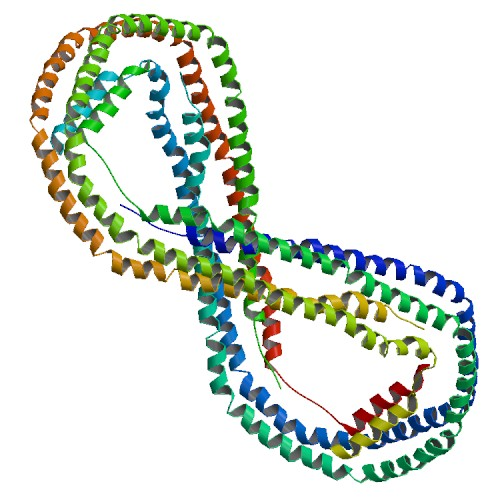
\includegraphics[width=0.4\textwidth]{images/PBB_Protein_APOA1_image.jpg}
    \caption{ApoA1 在蛋白质数据库 (PDB) 中的渲染结果}
\end{figure}

计算科学与高性能计算在当代科学研究和工程应用中扮演着至关重要的角色。
分子动力学模拟作为一种重要的计算科学工具,广泛用于模拟分子体系的行为,如生物分子、聚合物和材料。
其中,NAMD(NAnoscale Molecular Dynamics)\cite{phillips2005scalable}是一款广泛应用的分子动力学软件,其高度并行的特性使其成为模拟大规模分子系统的有力工具。
然而,目前,NAMD在国产CPU上的性能与一些国际竞争对手相比存在一定差距。


\begin{figure}[h]
    \centering
    
\includegraphics{images/namd-logo.png}
    \caption{NAMD 标识}
\end{figure}

本项目计划从 ApoA1 等蛋白质出发,在国产 CPU 上完成对这些蛋白质的分子动力学模拟计算,为国内科研和工程应用提供更高效的分子动力学模拟解决方案。
通过优化NAMD算法,我们将探讨如何充分利用国产CPU的硬件资源,提高模拟速度,降低计算成本,并使国内科研机构和工程部门能够更好地应对复杂的分子系统建模问题。

研究的意义在于不仅促进了分子动力学模拟的发展,还有助于推动国产CPU技术在科学计算领域的应用和发展。
这项研究将有助于提高我国在生物医药、材料科学、化学工程等领域的研究和创新水平,为国家自主研发计算机技术提供实际应用的范例。
最终,通过这项研究,我们将为国内高性能计算和科学研究社区提供一种有效的分子模拟工具,为我国的科学研究和工程应用带来巨大的潜在价值。

\section{国内外在该方向的研究现状及分析}

分子动力学在化学、医学方向的应用十分广泛。

% TODO:

NAMD 是一种开源高性能分子动力学模拟软件,用于模拟原子和分子之间的相互作用以及它们的运动行为。
NAMD的主要应用领域包括生物医学研究\cite{yao2020molecular}、生物化学\cite{knott2020characterization}、药物设计\cite{han2020computational}、材料科学和纳米技术。
这个软件的独特之处在于其能够模拟极小尺度的系统,如生物分子、蛋白质、DNA、聚合物和其他化学体系,以揭示它们的结构、动力学和相互作用。

% 国外,超算上的应用
% 2020 Gorden Bell 用了这个软件

% 国内
2010年,刘谦等人在中国科学院网络与信息中心深腾7000平台测试了 NAMD 的性能,并对STMV典型的烟草花叶卫星病毒进行了2048处理器核的模拟计算\cite{刘倩2010基于深腾}。
深腾计算机采取了采用混合架构的高性能计算集群,由 Intel Xeon 处理器集群与 Intel Itanium2 胖节点组成,主要采用的是 Intel 公司的 x86 指令集架构。
2017年,姚文军\cite{姚文军2017基于神威太湖之光的}等人将 NAMD 移植到了神威太湖之光上。

\section{主要研究内容}

本项目计划从 ApoA1 等蛋白质出发,在国产 CPU 上完成对这些蛋白质的分子动力学模拟计算。主要研究内容包括:

\subsection{蛋白质结构分析}

NAMD 主要用于蛋白质体系的分子动力学计算。
表 \ref{tab:protein-size} 中列出了一些蛋白质、大分子体系的原子数规模。
在计算前,需要获取蛋白质的基本结构数据,包括原子的数量和位置、环境参数等参数。

\subsection{分子动力学计算方式了解}

在进行计算前,需要了解分子动力学计算的基本原理,势函数与力场的概念,以及系综的选择方法。

\subsection{自主指令集架构了解与适应}

研究团队需要深入了解国产自主指令集架构,包括其体系结构特点、指令集编程模型和硬件特性。这将有助于更好地理解如何将 NAMD 移植到该架构上,并为后续的优化工作奠定基础。

\subsection{NAMD 移植工作}

将 NAMD 软件移植到国产自主指令集架构上,确保其在该架构上的基本运行。这包括适应指令集、调整编译工具链以支持目标架构,并解决与体系结构相关的兼容性问题。

\subsection{性能评估与基准测试}

对移植后的 NAMD 进行全面的性能评估,以了解在自主指令集架构上的性能表现。这包括运行基准测试和性能分析,以比较其与现有架构的性能差距。

\section{研究方案}

\subsection{调研蛋白质的性质与规模,收集蛋白质空间数据}

蛋白质的原子数目是影响分子动力学计算负载的关键。
载脂蛋白 A1 含有 92224 个原子,为小规模蛋白质。
其他一些蛋白质体系的原子数目在表 \ref{tab:protein-size} 中列出。

\begin{table}[h]
    \centering
    \caption{一些蛋白质、大分子体系的原子数规模}
    \label{tab:protein-size}
    \begin{tabular}{ccc}
        \toprule
        名称       & 简写     & 原子数目    \\
        \midrule
        载脂蛋白 A1  & ApoA1  & 92224   \\
        ATP合成酶   & ATPASE & 327506  \\
        卫星烟草花叶病毒 & STMV   & 1066628 \\
        \bottomrule
    \end{tabular}
\end{table}

除了蛋白质的性质规模外,还需研究蛋白质的三维结构数据。

蛋白质数据库(Protein Data Bank,简称PDB)\cite{burley2017protein,sussman1998protein} 是一个专门收录蛋白质及核酸的三维结构资料的数据库。
图 \ref{fig:protein-db} 展示了蛋白质数据库中蛋白质的一些例子。

可以从蛋白质数据库中下载所需要的蛋白质的原子位置信息,以及初始速度,格式为 PDB 文件。
另外,还需要蛋白质原子之间的成键信息,这些成键信息在 PSF 中储存。

表 \ref{tab:protein-files} 中列出了这两种信息文件。

\begin{table}[h]
    \centering
    \caption{从蛋白质数据库中下载的蛋白质信息文件}
    \label{tab:protein-files}
    \begin{tabular}{cc}
        \toprule
        格式  & 文件包含的信息  \\
        \midrule
        PDB & 原子位置、速度  \\
        PSF & 原子之间成键情况 \\
        \bottomrule
    \end{tabular}
\end{table}

\begin{figure}[h]
    \centering
    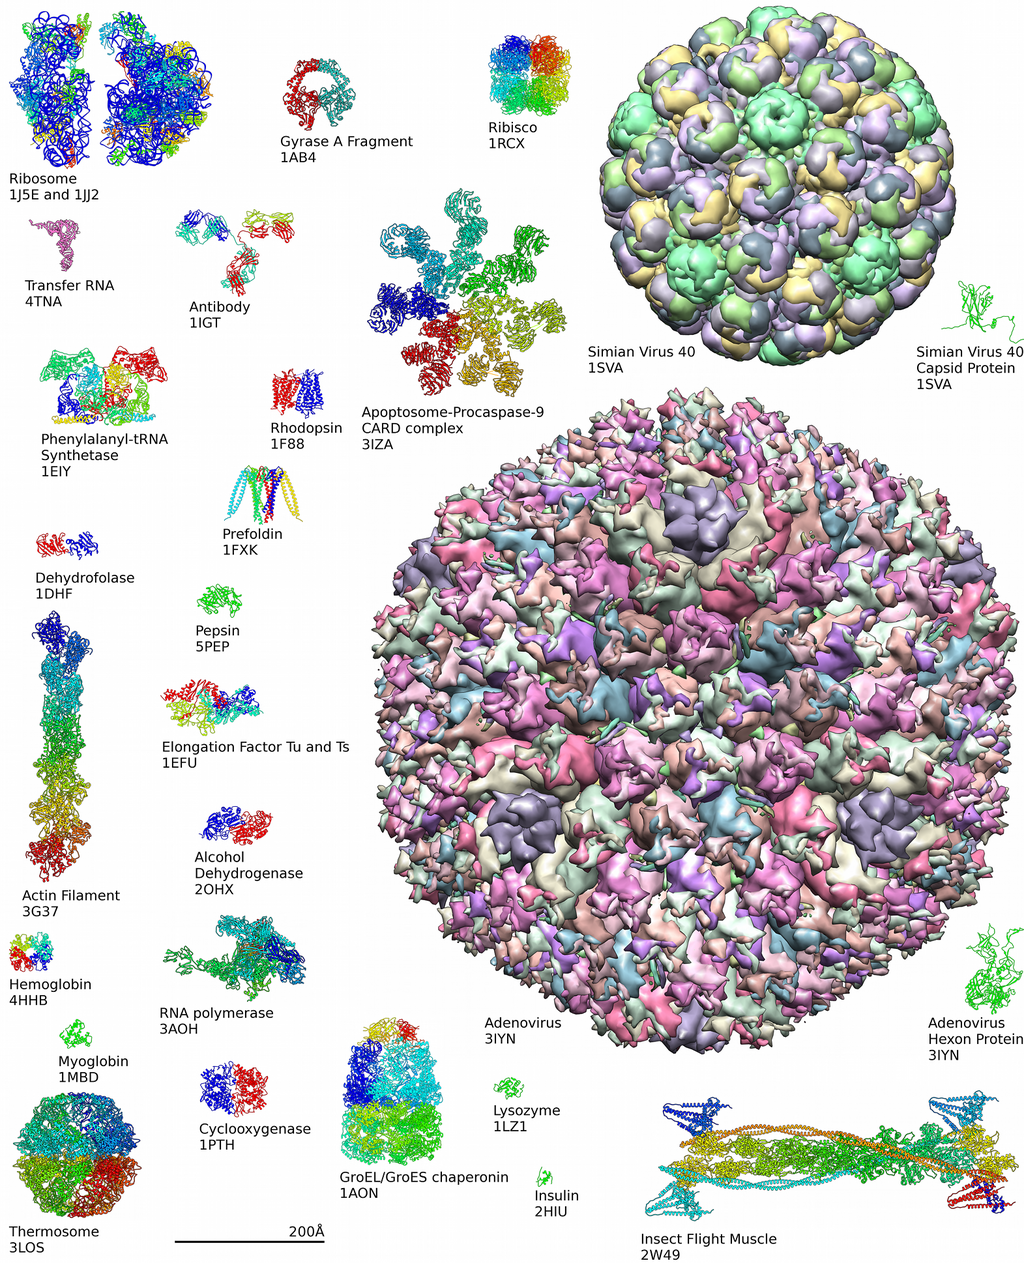
\includegraphics[width=0.35\textwidth]{images/1024px-Protein_structure_examples.png}
    \caption{蛋白质数据库(PDB)中蛋白质结构的一些例子。}
    \label{fig:protein-db}
\end{figure}

\subsection{分子动力学计算}

分子动力学计算的基本原理是对广义牛顿运动方程的求解。
系统的总势能为系统中各个原子的位置的函数 $U = (\vec{r_1}, \vec{r_2}, \dots, \vec{r_N})$。
在系统中的任意原子 $i$ ,根据牛顿力学,其受理和势函数关系为


\begin{equation}
    \vec{F} = -\nabla U (\vec{r_1}, \vec{r_2}, \dots, \vec{r_N}) = - \left( \vec{i} \frac{\partial}{\partial x_i} + \vec{j}\frac{\partial}{\partial x_y} + \vec{k} \frac{\partial}{\partial x_z}\right) U
\end{equation}

系统内任意原子的加速度和受力关系为\cite{易浩杰2019纳米静电喷射的分子动力学模拟研究}

\begin{equation}
    a_i = \frac{F_i}{m_i} = \frac{\mathrm{d}^2 r}{\mathrm{d} t^2}
\end{equation}

\subsection{国产 CPU 平台}

TODO

\subsection{优化方案分析}

\section{进度安排,预期达到的目标}

\begin{table}[h]
    \centering
    \caption{立项进度安排表}
    \begin{tabular}{cc}
        \toprule
        时间 (立项时间为 $T_1$) & 进度                              \\
        \midrule
        $T_1$ + 1 月      & 蛋白质数据库收集与了解                     \\
        $T_1$ + 3 月      & NAMD 在 Intel CPU 上的蛋白质计算模拟      \\
        $T_1$ + 6 月      & NAMD 在 国产 CPU 上的初步移植与正确性验证 中期检查 \\
        $T_1$ + 9 月      & 蛋白质在国产 CPU 上的模拟和优化              \\
        $T_1$ + 12 月     & 项目结题                            \\
        \bottomrule
    \end{tabular}
\end{table}
\section{课题已具备和所需的条件、经费}
\section{研究过程中可能遇到的困难和问题,解决的措施}
\section{主要参考文献}
\bibliographystyle{hithesis}
\bibliography{reference}

% Local Variables:
% TeX-master: "../mainart"
% TeX-engine: xetex
% End:
